\titleimage{
	\centering
	%	%Folgende Box kann selbstverständlich durch ein mit \includegraphics geladenes Bild ersetzt werden.
	\bigskip
	\bigskip
	\bigskip
	\bigskip
	\bigskip
	\bigskip
	\bigskip
	\bigskip
	\bigskip
	\bigskip
%	\bigskip	
	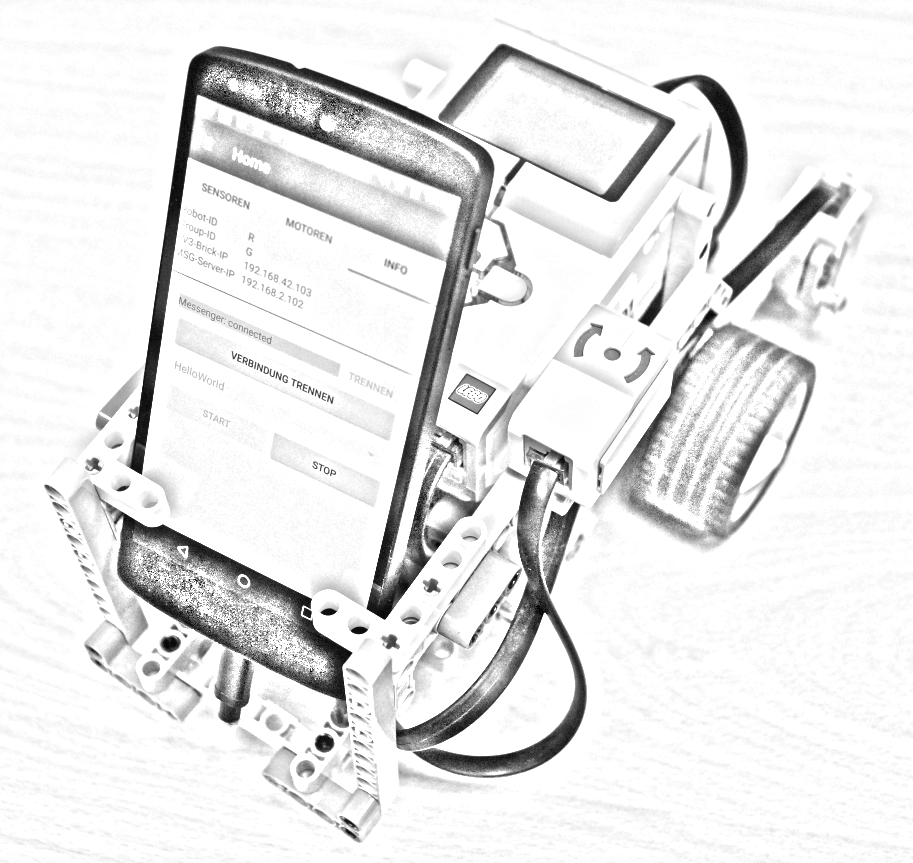
\includegraphics[width=0.8\textwidth]{MindroidTitle.png}
	%\color{black!30}\rule{\width}{\height}
}


%Varianten der Infoboxen
\addTitleBox{\includegraphics[width=\linewidth]{../ist_logo.pdf}}
%\addTitleBoxLogo{example-image}
%\addTitleBoxLogo*{\includegraphics[width=.3\linewidth]{example-image}}
	
	
	
	\newcommand{\titletext}{No Title - No Content}
	
	\ifthenelse{\boolean{doc}}{
		\renewcommand{\titletext}{Dokumentation}
	}{}
	\ifthenelse{\boolean{devDoc}}{
		\renewcommand{\titletext}{Entwickler-Dokumentation}
	}{}
	
	\ifthenelse{\boolean{tasks}}{
		\ifthenelse{\boolean{solution}}{
			\renewcommand{\titletext}{Aufgabenstellung \\mit Lösungen}
		}{
			\renewcommand{\titletext}{Aufgabenstellung}
		}
	}{
		\ifthenelse{\boolean{solution}}{
			\renewcommand{\titletext}{Lösungen}
		}{}
	}


	\pagenumbering{arabic}	
	\title{Mindroid Workshop \\ \titletext}
	\subtitle{NeXT Generation on Campus\newline TU Darmstadt}
%	\subsubtitle{}
	
	\maketitle	
	
	\ifthenelse{\boolean{solution}}{
		\centering	
		\bigskip\bigskip\bigskip\bigskip\bigskip\bigskip\bigskip\bigskip\bigskip	
		{\Huge LÖSUNGEN}
		\newpage
	}{	
%	\bigskip\bigskip\bigskip\bigskip\bigskip
%		\easygcenter{.9\textwidth}{logo/MindroidTitle.png}
%		\newpage
}